\documentclass[twoside]{book}

% Packages required by doxygen
\usepackage{calc}
\usepackage{doxygen}
\usepackage{graphicx}
\usepackage[utf8]{inputenc}
\usepackage{makeidx}
\usepackage{multicol}
\usepackage{multirow}
\usepackage{textcomp}
\usepackage[table]{xcolor}

% Font selection
\usepackage[T1]{fontenc}
\usepackage{mathptmx}
\usepackage[scaled=.90]{helvet}
\usepackage{courier}
\usepackage{amssymb}
\usepackage{sectsty}
\renewcommand{\familydefault}{\sfdefault}
\allsectionsfont{%
  \fontseries{bc}\selectfont%
  \color{darkgray}%
}
\renewcommand{\DoxyLabelFont}{%
  \fontseries{bc}\selectfont%
  \color{darkgray}%
}

% Page & text layout
\usepackage{geometry}
\geometry{%
  a4paper,%
  top=2.5cm,%
  bottom=2.5cm,%
  left=2.5cm,%
  right=2.5cm%
}
\tolerance=750
\hfuzz=15pt
\hbadness=750
\setlength{\emergencystretch}{15pt}
\setlength{\parindent}{0cm}
\setlength{\parskip}{0.2cm}
\makeatletter
\renewcommand{\paragraph}{%
  \@startsection{paragraph}{4}{0ex}{-1.0ex}{1.0ex}{%
    \normalfont\normalsize\bfseries\SS@parafont%
  }%
}
\renewcommand{\subparagraph}{%
  \@startsection{subparagraph}{5}{0ex}{-1.0ex}{1.0ex}{%
    \normalfont\normalsize\bfseries\SS@subparafont%
  }%
}
\makeatother

% Headers & footers
\usepackage{fancyhdr}
\pagestyle{fancyplain}
\fancyhead[LE]{\fancyplain{}{\bfseries\thepage}}
\fancyhead[CE]{\fancyplain{}{}}
\fancyhead[RE]{\fancyplain{}{\bfseries\leftmark}}
\fancyhead[LO]{\fancyplain{}{\bfseries\rightmark}}
\fancyhead[CO]{\fancyplain{}{}}
\fancyhead[RO]{\fancyplain{}{\bfseries\thepage}}
\fancyfoot[LE]{\fancyplain{}{}}
\fancyfoot[CE]{\fancyplain{}{}}
\fancyfoot[RE]{\fancyplain{}{\bfseries\scriptsize Generated on Wed Sep 30 2015 02\-:13\-:45 for My Project by Doxygen }}
\fancyfoot[LO]{\fancyplain{}{\bfseries\scriptsize Generated on Wed Sep 30 2015 02\-:13\-:45 for My Project by Doxygen }}
\fancyfoot[CO]{\fancyplain{}{}}
\fancyfoot[RO]{\fancyplain{}{}}
\renewcommand{\footrulewidth}{0.4pt}
\renewcommand{\chaptermark}[1]{%
  \markboth{#1}{}%
}
\renewcommand{\sectionmark}[1]{%
  \markright{\thesection\ #1}%
}

% Indices & bibliography
\usepackage{natbib}
\usepackage[titles]{tocloft}
\setcounter{tocdepth}{3}
\setcounter{secnumdepth}{5}
\makeindex

% Hyperlinks (required, but should be loaded last)
\usepackage{ifpdf}
\ifpdf
  \usepackage[pdftex,pagebackref=true]{hyperref}
\else
  \usepackage[ps2pdf,pagebackref=true]{hyperref}
\fi
\hypersetup{%
  colorlinks=true,%
  linkcolor=blue,%
  citecolor=blue,%
  unicode%
}

% Custom commands
\newcommand{\clearemptydoublepage}{%
  \newpage{\pagestyle{empty}\cleardoublepage}%
}


%===== C O N T E N T S =====

\begin{document}

% Titlepage & ToC
\hypersetup{pageanchor=false}
\pagenumbering{roman}
\begin{titlepage}
\vspace*{7cm}
\begin{center}%
{\Large My Project }\\
\vspace*{1cm}
{\large Generated by Doxygen 1.8.6}\\
\vspace*{0.5cm}
{\small Wed Sep 30 2015 02:13:45}\\
\end{center}
\end{titlepage}
\clearemptydoublepage
\tableofcontents
\clearemptydoublepage
\pagenumbering{arabic}
\hypersetup{pageanchor=true}

%--- Begin generated contents ---
\chapter{Namespace Index}
\section{Namespace List}
Here is a list of all namespaces with brief descriptions\-:\begin{DoxyCompactList}
\item\contentsline{section}{\hyperlink{namespacevideorentalsystem}{videorentalsystem} }{\pageref{namespacevideorentalsystem}}{}
\end{DoxyCompactList}

\chapter{Hierarchical Index}
\section{Class Hierarchy}
This inheritance list is sorted roughly, but not completely, alphabetically\-:\begin{DoxyCompactList}
\item \contentsline{section}{carcruisecontrolsystem.\-Car\-Cruise\-Control\-System}{\pageref{classcarcruisecontrolsystem_1_1CarCruiseControlSystem}}{}
\item J\-Frame\begin{DoxyCompactList}
\item \contentsline{section}{carcruisecontrolsystem.\-Control}{\pageref{classcarcruisecontrolsystem_1_1Control}}{}
\item \contentsline{section}{carcruisecontrolsystem.\-Greeter}{\pageref{classcarcruisecontrolsystem_1_1Greeter}}{}
\end{DoxyCompactList}
\end{DoxyCompactList}

\chapter{Class Index}
\section{Class List}
Here are the classes, structs, unions and interfaces with brief descriptions\-:\begin{DoxyCompactList}
\item\contentsline{section}{\hyperlink{classcarcruisecontrolsystem_1_1CarCruiseControlSystem}{carcruisecontrolsystem.\-Car\-Cruise\-Control\-System} }{\pageref{classcarcruisecontrolsystem_1_1CarCruiseControlSystem}}{}
\item\contentsline{section}{\hyperlink{classcarcruisecontrolsystem_1_1Control}{carcruisecontrolsystem.\-Control} }{\pageref{classcarcruisecontrolsystem_1_1Control}}{}
\item\contentsline{section}{\hyperlink{classcarcruisecontrolsystem_1_1Greeter}{carcruisecontrolsystem.\-Greeter} }{\pageref{classcarcruisecontrolsystem_1_1Greeter}}{}
\end{DoxyCompactList}

\chapter{File Index}
\section{File List}
Here is a list of all files with brief descriptions\-:\begin{DoxyCompactList}
\item\contentsline{section}{\hyperlink{CostData_8java}{Cost\-Data.\-java} }{\pageref{CostData_8java}}{}
\item\contentsline{section}{\hyperlink{Costumer_8java}{Costumer.\-java} }{\pageref{Costumer_8java}}{}
\item\contentsline{section}{\hyperlink{CostumerForm_8java}{Costumer\-Form.\-java} }{\pageref{CostumerForm_8java}}{}
\item\contentsline{section}{\hyperlink{Movie_8java}{Movie.\-java} }{\pageref{Movie_8java}}{}
\item\contentsline{section}{\hyperlink{Producer_8java}{Producer.\-java} }{\pageref{Producer_8java}}{}
\item\contentsline{section}{\hyperlink{Rental_8java}{Rental.\-java} }{\pageref{Rental_8java}}{}
\item\contentsline{section}{\hyperlink{RentVideo_8java}{Rent\-Video.\-java} }{\pageref{RentVideo_8java}}{}
\item\contentsline{section}{\hyperlink{VideoData_8java}{Video\-Data.\-java} }{\pageref{VideoData_8java}}{}
\item\contentsline{section}{\hyperlink{VideoForm_8java}{Video\-Form.\-java} }{\pageref{VideoForm_8java}}{}
\item\contentsline{section}{\hyperlink{VideoRentalSystem_8java}{Video\-Rental\-System.\-java} }{\pageref{VideoRentalSystem_8java}}{}
\item\contentsline{section}{\hyperlink{Welcome_8java}{Welcome.\-java} }{\pageref{Welcome_8java}}{}
\end{DoxyCompactList}

\chapter{Namespace Documentation}
\hypertarget{namespacecarcruisecontrolsystem}{\section{Package carcruisecontrolsystem}
\label{namespacecarcruisecontrolsystem}\index{carcruisecontrolsystem@{carcruisecontrolsystem}}
}
\subsection*{Classes}
\begin{DoxyCompactItemize}
\item 
class \hyperlink{classcarcruisecontrolsystem_1_1CarCruiseControlSystem}{Car\-Cruise\-Control\-System}
\item 
class \hyperlink{classcarcruisecontrolsystem_1_1Control}{Control}
\item 
class \hyperlink{classcarcruisecontrolsystem_1_1Greeter}{Greeter}
\end{DoxyCompactItemize}

\chapter{Class Documentation}
\hypertarget{classcarcruisecontrolsystem_1_1CarCruiseControlSystem}{\section{carcruisecontrolsystem.\-Car\-Cruise\-Control\-System Class Reference}
\label{classcarcruisecontrolsystem_1_1CarCruiseControlSystem}\index{carcruisecontrolsystem.\-Car\-Cruise\-Control\-System@{carcruisecontrolsystem.\-Car\-Cruise\-Control\-System}}
}


Collaboration diagram for carcruisecontrolsystem.\-Car\-Cruise\-Control\-System\-:
\nopagebreak
\begin{figure}[H]
\begin{center}
\leavevmode
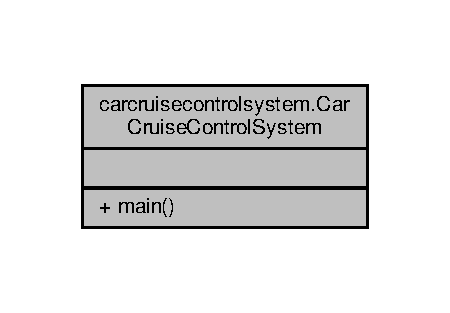
\includegraphics[width=216pt]{classcarcruisecontrolsystem_1_1CarCruiseControlSystem__coll__graph}
\end{center}
\end{figure}
\subsection*{Static Public Member Functions}
\begin{DoxyCompactItemize}
\item 
static void \hyperlink{classcarcruisecontrolsystem_1_1CarCruiseControlSystem_a1b0191a072782fe47df5d837c2d2401f}{main} (String\mbox{[}$\,$\mbox{]} args)
\end{DoxyCompactItemize}


\subsection{Detailed Description}
\begin{DoxyAuthor}{Author}
abhinav 
\end{DoxyAuthor}


\subsection{Member Function Documentation}
\hypertarget{classcarcruisecontrolsystem_1_1CarCruiseControlSystem_a1b0191a072782fe47df5d837c2d2401f}{\index{carcruisecontrolsystem\-::\-Car\-Cruise\-Control\-System@{carcruisecontrolsystem\-::\-Car\-Cruise\-Control\-System}!main@{main}}
\index{main@{main}!carcruisecontrolsystem::CarCruiseControlSystem@{carcruisecontrolsystem\-::\-Car\-Cruise\-Control\-System}}
\subsubsection[{main}]{\setlength{\rightskip}{0pt plus 5cm}static void carcruisecontrolsystem.\-Car\-Cruise\-Control\-System.\-main (
\begin{DoxyParamCaption}
\item[{String\mbox{[}$\,$\mbox{]}}]{args}
\end{DoxyParamCaption}
)\hspace{0.3cm}{\ttfamily [inline]}, {\ttfamily [static]}}}\label{classcarcruisecontrolsystem_1_1CarCruiseControlSystem_a1b0191a072782fe47df5d837c2d2401f}

\begin{DoxyParams}{Parameters}
{\em args} & the command line arguments \\
\hline
\end{DoxyParams}


The documentation for this class was generated from the following file\-:\begin{DoxyCompactItemize}
\item 
\hyperlink{CarCruiseControlSystem_8java}{Car\-Cruise\-Control\-System.\-java}\end{DoxyCompactItemize}

\hypertarget{classcarcruisecontrolsystem_1_1Control}{\section{carcruisecontrolsystem.\-Control Class Reference}
\label{classcarcruisecontrolsystem_1_1Control}\index{carcruisecontrolsystem.\-Control@{carcruisecontrolsystem.\-Control}}
}


Inheritance diagram for carcruisecontrolsystem.\-Control\-:
\nopagebreak
\begin{figure}[H]
\begin{center}
\leavevmode
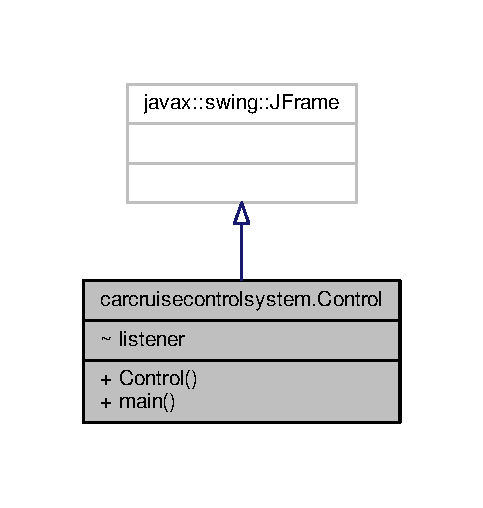
\includegraphics[width=232pt]{classcarcruisecontrolsystem_1_1Control__inherit__graph}
\end{center}
\end{figure}


Collaboration diagram for carcruisecontrolsystem.\-Control\-:
\nopagebreak
\begin{figure}[H]
\begin{center}
\leavevmode
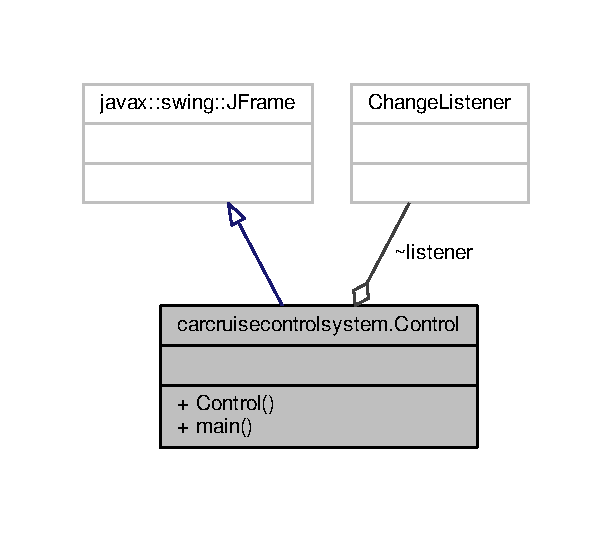
\includegraphics[width=293pt]{classcarcruisecontrolsystem_1_1Control__coll__graph}
\end{center}
\end{figure}
\subsection*{Public Member Functions}
\begin{DoxyCompactItemize}
\item 
\hyperlink{classcarcruisecontrolsystem_1_1Control_af3cae43a2b98050495daf14efd567447}{Control} ()
\end{DoxyCompactItemize}
\subsection*{Static Public Member Functions}
\begin{DoxyCompactItemize}
\item 
static void \hyperlink{classcarcruisecontrolsystem_1_1Control_ab04b1fccda59127ec19a9d0df2db306b}{main} (String args\mbox{[}$\,$\mbox{]})
\end{DoxyCompactItemize}


\subsection{Detailed Description}
\begin{DoxyAuthor}{Author}
abhinav 
\end{DoxyAuthor}


\subsection{Constructor \& Destructor Documentation}
\hypertarget{classcarcruisecontrolsystem_1_1Control_af3cae43a2b98050495daf14efd567447}{\index{carcruisecontrolsystem\-::\-Control@{carcruisecontrolsystem\-::\-Control}!Control@{Control}}
\index{Control@{Control}!carcruisecontrolsystem::Control@{carcruisecontrolsystem\-::\-Control}}
\subsubsection[{Control}]{\setlength{\rightskip}{0pt plus 5cm}carcruisecontrolsystem.\-Control.\-Control (
\begin{DoxyParamCaption}
{}
\end{DoxyParamCaption}
)\hspace{0.3cm}{\ttfamily [inline]}}}\label{classcarcruisecontrolsystem_1_1Control_af3cae43a2b98050495daf14efd567447}


\subsection{Member Function Documentation}
\hypertarget{classcarcruisecontrolsystem_1_1Control_ab04b1fccda59127ec19a9d0df2db306b}{\index{carcruisecontrolsystem\-::\-Control@{carcruisecontrolsystem\-::\-Control}!main@{main}}
\index{main@{main}!carcruisecontrolsystem::Control@{carcruisecontrolsystem\-::\-Control}}
\subsubsection[{main}]{\setlength{\rightskip}{0pt plus 5cm}static void carcruisecontrolsystem.\-Control.\-main (
\begin{DoxyParamCaption}
\item[{String}]{args\mbox{[}$\,$\mbox{]}}
\end{DoxyParamCaption}
)\hspace{0.3cm}{\ttfamily [inline]}, {\ttfamily [static]}}}\label{classcarcruisecontrolsystem_1_1Control_ab04b1fccda59127ec19a9d0df2db306b}

\begin{DoxyParams}{Parameters}
{\em args} & the command line arguments \\
\hline
\end{DoxyParams}


The documentation for this class was generated from the following file\-:\begin{DoxyCompactItemize}
\item 
\hyperlink{Control_8java}{Control.\-java}\end{DoxyCompactItemize}

\hypertarget{classcarcruisecontrolsystem_1_1Greeter}{\section{carcruisecontrolsystem.\-Greeter Class Reference}
\label{classcarcruisecontrolsystem_1_1Greeter}\index{carcruisecontrolsystem.\-Greeter@{carcruisecontrolsystem.\-Greeter}}
}


Inheritance diagram for carcruisecontrolsystem.\-Greeter\-:
\nopagebreak
\begin{figure}[H]
\begin{center}
\leavevmode
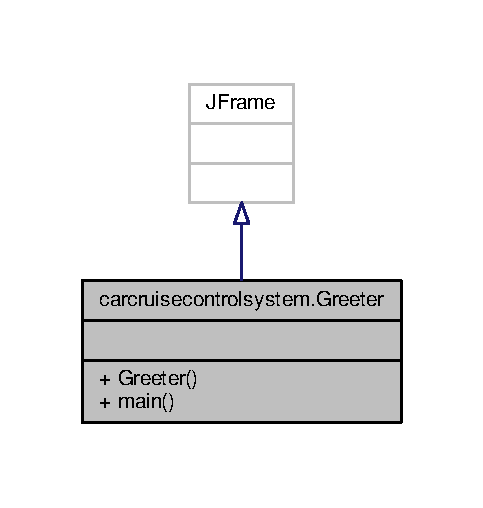
\includegraphics[width=232pt]{classcarcruisecontrolsystem_1_1Greeter__inherit__graph}
\end{center}
\end{figure}


Collaboration diagram for carcruisecontrolsystem.\-Greeter\-:
\nopagebreak
\begin{figure}[H]
\begin{center}
\leavevmode
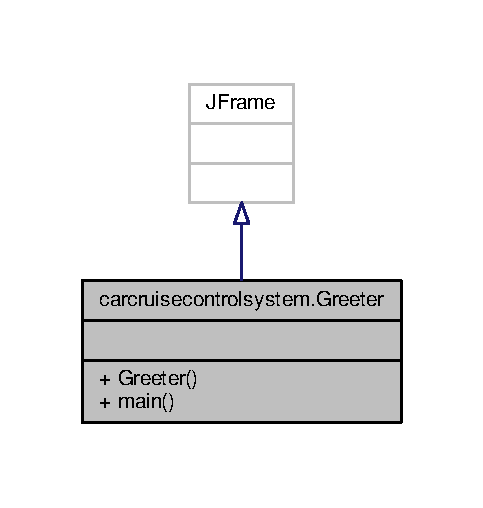
\includegraphics[width=232pt]{classcarcruisecontrolsystem_1_1Greeter__coll__graph}
\end{center}
\end{figure}
\subsection*{Public Member Functions}
\begin{DoxyCompactItemize}
\item 
\hyperlink{classcarcruisecontrolsystem_1_1Greeter_a404dfadee4c1d8cff268ae192dade8be}{Greeter} ()
\end{DoxyCompactItemize}
\subsection*{Static Public Member Functions}
\begin{DoxyCompactItemize}
\item 
static void \hyperlink{classcarcruisecontrolsystem_1_1Greeter_a501765e776e0fc3423d1200df8cfc5bc}{main} (String args\mbox{[}$\,$\mbox{]})
\end{DoxyCompactItemize}


\subsection{Detailed Description}
\begin{DoxyAuthor}{Author}
abhinav 
\end{DoxyAuthor}


\subsection{Constructor \& Destructor Documentation}
\hypertarget{classcarcruisecontrolsystem_1_1Greeter_a404dfadee4c1d8cff268ae192dade8be}{\index{carcruisecontrolsystem\-::\-Greeter@{carcruisecontrolsystem\-::\-Greeter}!Greeter@{Greeter}}
\index{Greeter@{Greeter}!carcruisecontrolsystem::Greeter@{carcruisecontrolsystem\-::\-Greeter}}
\subsubsection[{Greeter}]{\setlength{\rightskip}{0pt plus 5cm}carcruisecontrolsystem.\-Greeter.\-Greeter (
\begin{DoxyParamCaption}
{}
\end{DoxyParamCaption}
)\hspace{0.3cm}{\ttfamily [inline]}}}\label{classcarcruisecontrolsystem_1_1Greeter_a404dfadee4c1d8cff268ae192dade8be}
Creates new form \hyperlink{classcarcruisecontrolsystem_1_1Greeter}{Greeter} 

\subsection{Member Function Documentation}
\hypertarget{classcarcruisecontrolsystem_1_1Greeter_a501765e776e0fc3423d1200df8cfc5bc}{\index{carcruisecontrolsystem\-::\-Greeter@{carcruisecontrolsystem\-::\-Greeter}!main@{main}}
\index{main@{main}!carcruisecontrolsystem::Greeter@{carcruisecontrolsystem\-::\-Greeter}}
\subsubsection[{main}]{\setlength{\rightskip}{0pt plus 5cm}static void carcruisecontrolsystem.\-Greeter.\-main (
\begin{DoxyParamCaption}
\item[{String}]{args\mbox{[}$\,$\mbox{]}}
\end{DoxyParamCaption}
)\hspace{0.3cm}{\ttfamily [inline]}, {\ttfamily [static]}}}\label{classcarcruisecontrolsystem_1_1Greeter_a501765e776e0fc3423d1200df8cfc5bc}

\begin{DoxyParams}{Parameters}
{\em args} & the command line arguments \\
\hline
\end{DoxyParams}


The documentation for this class was generated from the following file\-:\begin{DoxyCompactItemize}
\item 
\hyperlink{Greeter_8java}{Greeter.\-java}\end{DoxyCompactItemize}

\chapter{File Documentation}
\hypertarget{CarCruiseControlSystem_8java}{\section{Car\-Cruise\-Control\-System.\-java File Reference}
\label{CarCruiseControlSystem_8java}\index{Car\-Cruise\-Control\-System.\-java@{Car\-Cruise\-Control\-System.\-java}}
}
\subsection*{Classes}
\begin{DoxyCompactItemize}
\item 
class \hyperlink{classcarcruisecontrolsystem_1_1CarCruiseControlSystem}{carcruisecontrolsystem.\-Car\-Cruise\-Control\-System}
\end{DoxyCompactItemize}
\subsection*{Packages}
\begin{DoxyCompactItemize}
\item 
package \hyperlink{namespacecarcruisecontrolsystem}{carcruisecontrolsystem}
\end{DoxyCompactItemize}

\hypertarget{Control_8java}{\section{Control.\-java File Reference}
\label{Control_8java}\index{Control.\-java@{Control.\-java}}
}
\subsection*{Classes}
\begin{DoxyCompactItemize}
\item 
class \hyperlink{classcarcruisecontrolsystem_1_1Control}{carcruisecontrolsystem.\-Control}
\end{DoxyCompactItemize}
\subsection*{Packages}
\begin{DoxyCompactItemize}
\item 
package \hyperlink{namespacecarcruisecontrolsystem}{carcruisecontrolsystem}
\end{DoxyCompactItemize}

\hypertarget{Greeter_8java}{\section{Greeter.\-java File Reference}
\label{Greeter_8java}\index{Greeter.\-java@{Greeter.\-java}}
}
\subsection*{Classes}
\begin{DoxyCompactItemize}
\item 
class \hyperlink{classcarcruisecontrolsystem_1_1Greeter}{carcruisecontrolsystem.\-Greeter}
\end{DoxyCompactItemize}
\subsection*{Packages}
\begin{DoxyCompactItemize}
\item 
package \hyperlink{namespacecarcruisecontrolsystem}{carcruisecontrolsystem}
\end{DoxyCompactItemize}

%--- End generated contents ---

% Index
\newpage
\phantomsection
\addcontentsline{toc}{chapter}{Index}
\printindex

\end{document}
